\documentclass[10pt,a4paper]{article}
\usepackage[latin1]{inputenc}
\usepackage{amsmath}
\usepackage{amsfonts}
\usepackage{amssymb}
\usepackage{graphicx}
\usepackage{float}
\usepackage{soul}
\usepackage{caption}
\usepackage{subcaption}
\usepackage[section]{placeins}
\usepackage[left=2cm,right=2cm,top=2cm,bottom=2cm]{geometry}
\author{Akshat Mahajan}
\title{Physics 180Q - Lab Report 3}
\begin{document}
\maketitle

\textsl{This lab was performed in conjunction with Hanwen Qin. The variable impedance terminator was set to 10 k$\Omega$ throughout, as analysis of the results from Week 1 had demonstrated that it gave the most accurate responses overall.}

\section*{Part 1: Build An Electric Eye}

We built a CCD system using a C-mount adapter, ND filter, and adjustable lens holder. The focal length of the lens was 30 mm. We focused it on images on the far side of the room.
\begin{figure}[h]
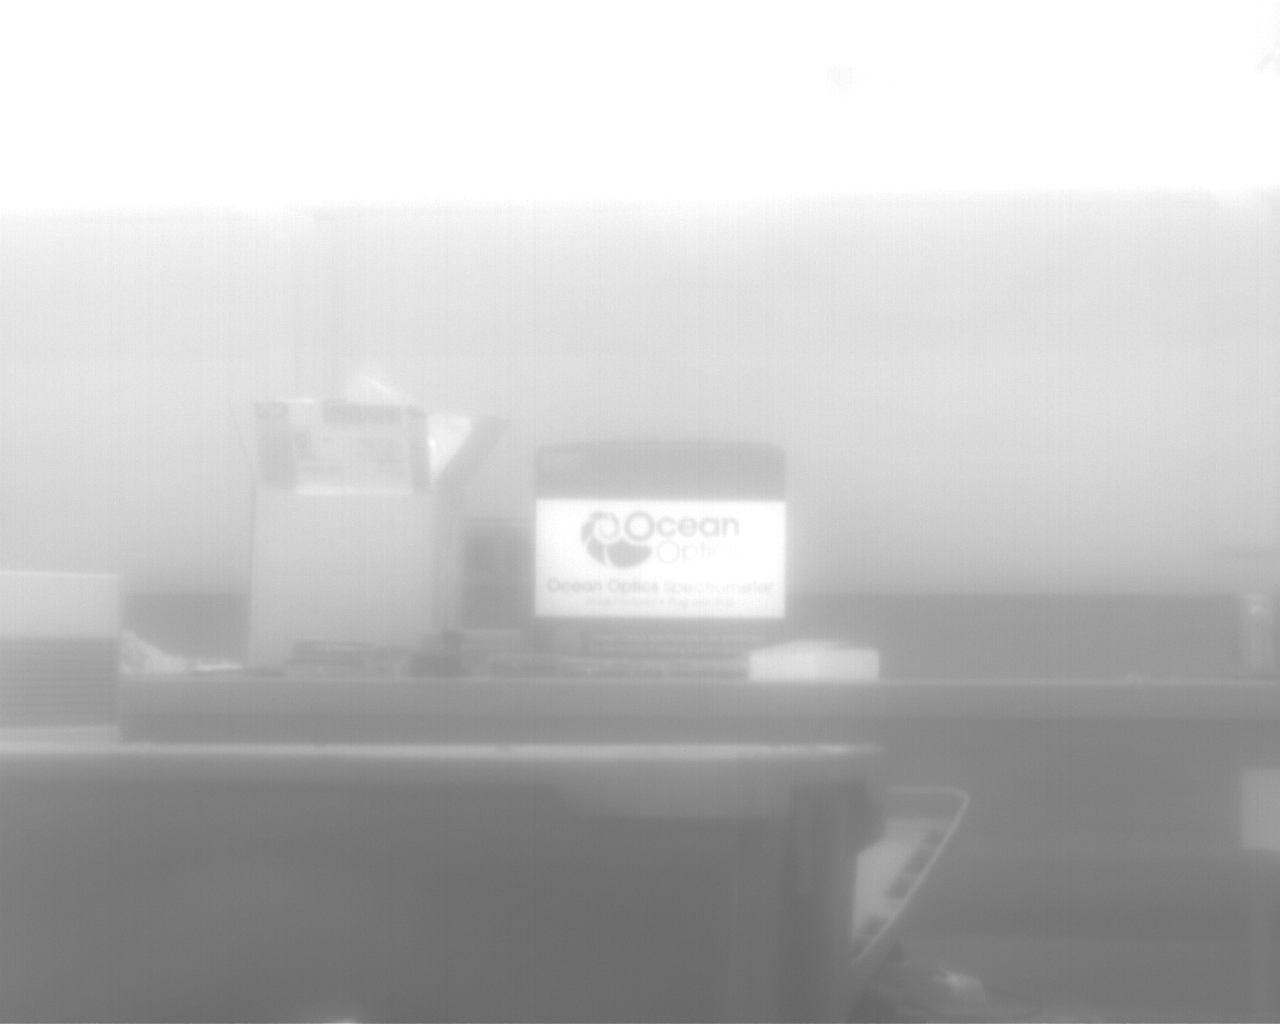
\includegraphics[width=\textwidth]{../Analysis/Part1-Run1.png}
\caption{Image obtained from electric eye of far side of the room.} 
\end{figure}

\section*{Part 2: Build A Telescope}
We built a telescope out of a tube length of 110 mm, an objective of focal length 75 mm, and an eyepiece of focal length 33 mm. We focused on the same box as shown in Part 1.\\
\\
The magnification obtained was only $\dfrac{-f_{0}}{f_{e}} = \dfrac{-75}{33} = -2.27$. This can be verified by measuring the length of the box as it appears in Figure 1 and the length of the box in Figure 2. The negative sign indicates inversion.\\
\\
The relevant ray-tracing proof of concept can be found in the accompanying Prelab 3.
\begin{figure}[h]
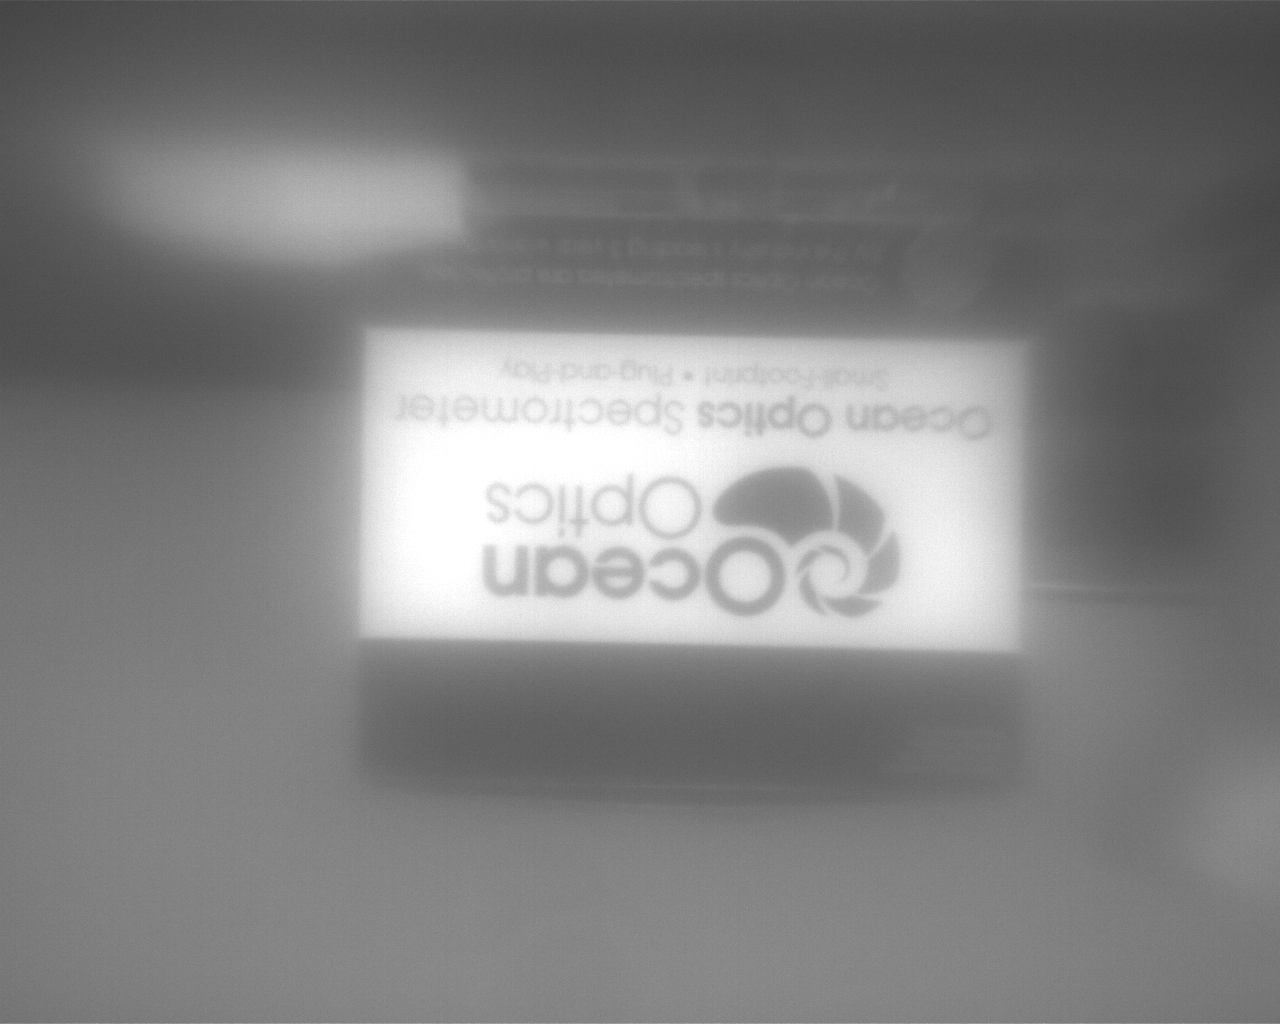
\includegraphics[width=\textwidth]{../Analysis/Part2.png}
\caption{Image obtained from telescope of far side of the room.} 
\end{figure}
\section*{Part 3: Build A Microscope}
We built a microscope out of a tube length of 110 mm, an objective of focal length 35 mm, and an eyepiece of focal length 53 mm. We focused on the same box as shown in Part 1. The trick here is to have both the objective's focal length exceed the eyepiece's as well as to ensure that the sum did not equal or exceed the tube length.\\
\\
The magnification obtained this way can be shown to be $$M = \dfrac{-L}{f_{0}}\times\dfrac{30\mathrm{mm}}{f_{e}} = \dfrac{110}{35}\times\dfrac{30}{53} = 1.77$$ Typically, a value of 25 cm is used to indicate the focal length of the eye, but in this case the focal length of our electric eye is 30 mm. The negative sign indicates inversion.\\
\\
The relevant ray-tracing proof of concept was inspired by Justin.
\begin{figure}[t]
\begin{subfigure}{0.5\textwidth}
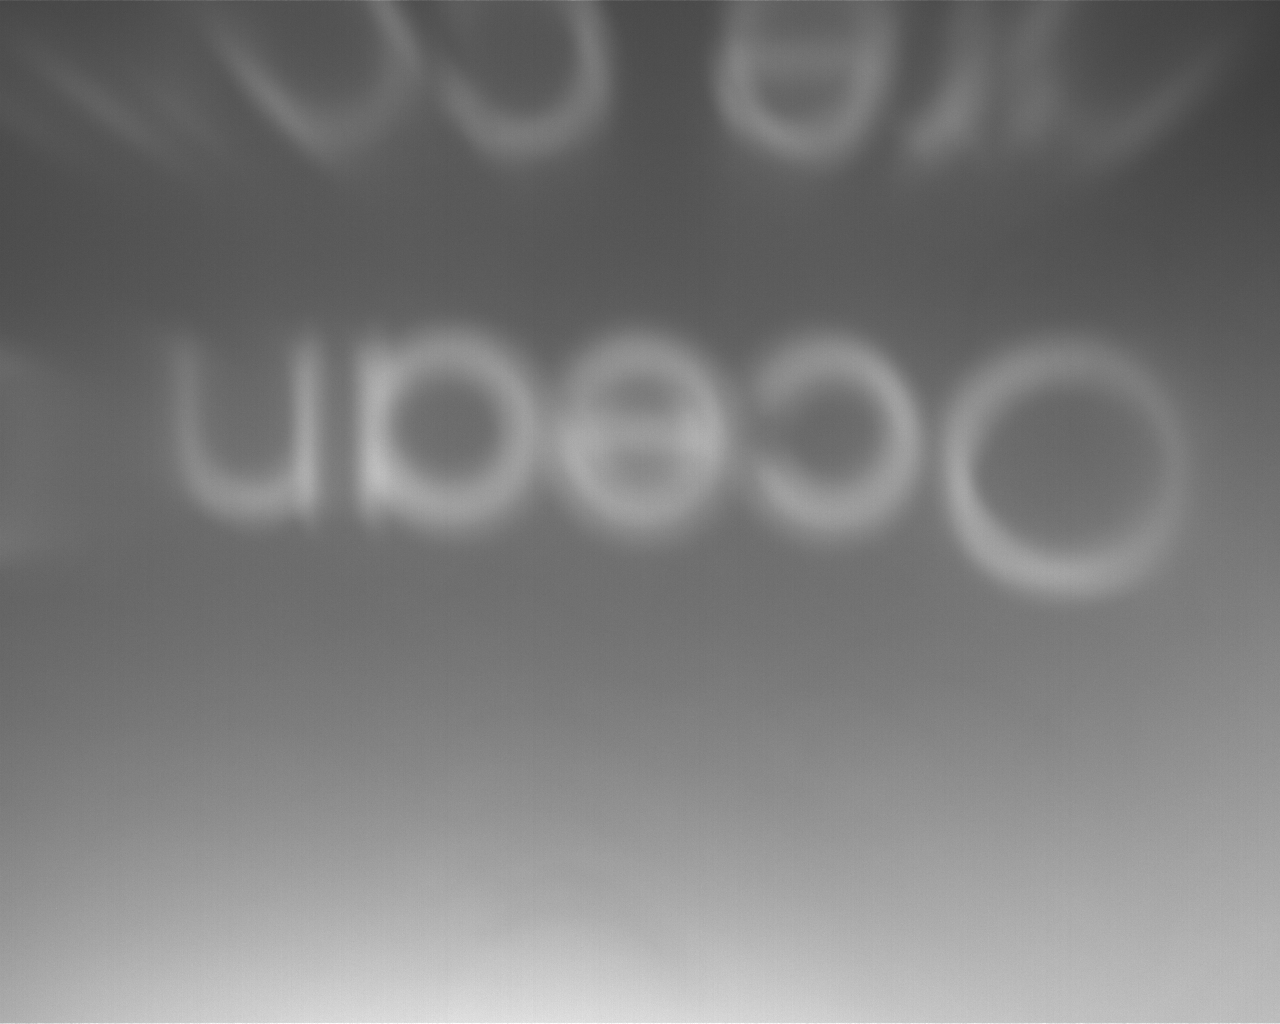
\includegraphics[width=\textwidth]{../Analysis/Part3-Run5.png}
\end{subfigure}
\begin{subfigure}{0.5\textwidth}
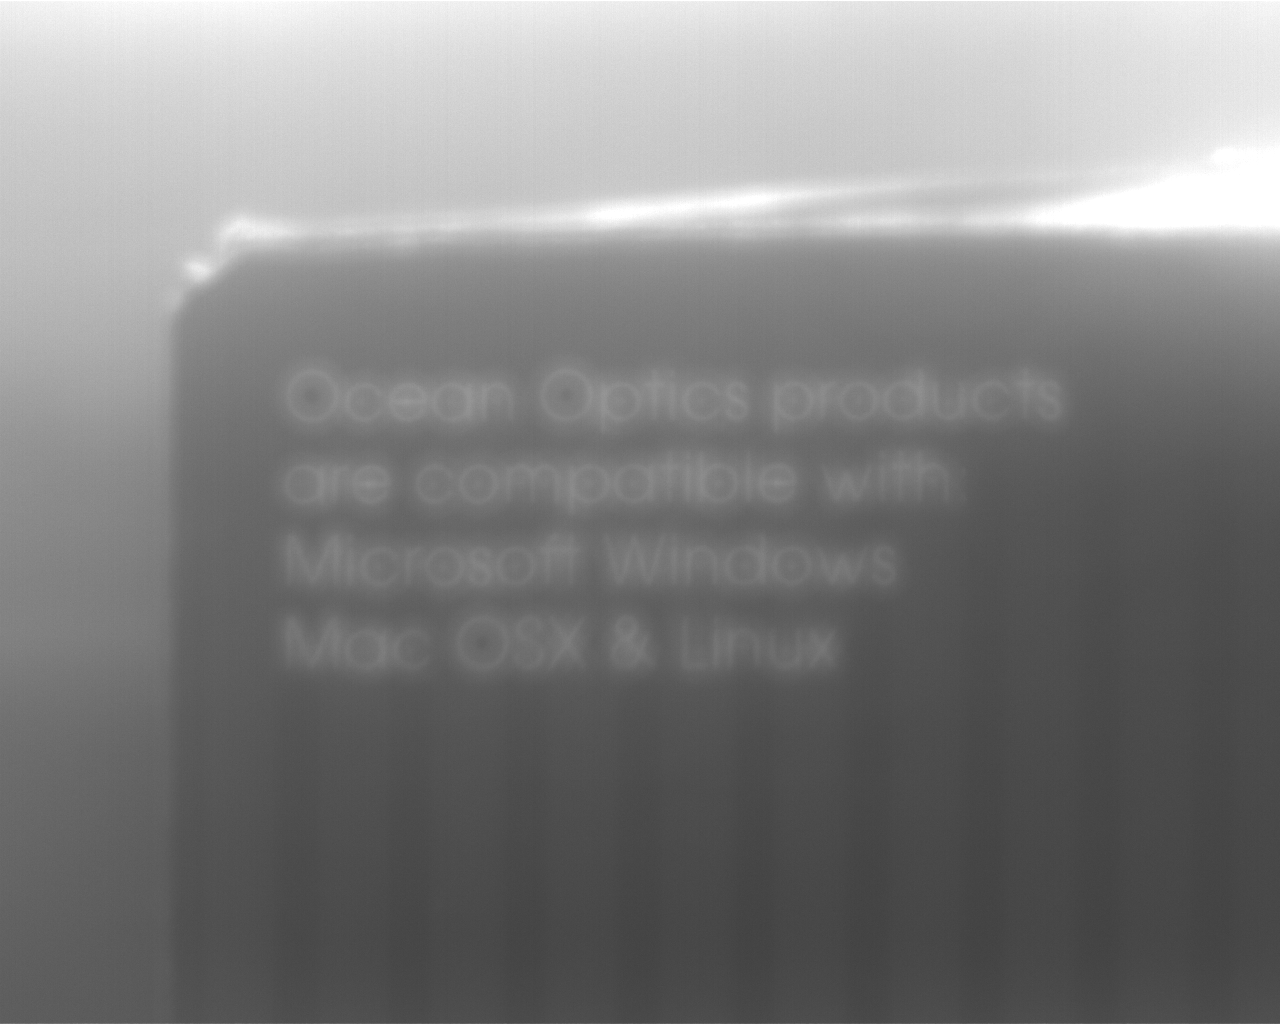
\includegraphics[width=\textwidth]{../Analysis/Part3-Run3.png}
\end{subfigure}
\caption{\textsl{Right:} Photograph of image without microscope. \textsl{Left:} Same image with microscope.}
\end{figure}
\section*{Part 4: Measure The Beam Profile}
We separated the beam from the photodiode by the length of our optical table. We then marked positions at 50 mm away from the beam shutter, then 381 mm after the first shutter, and finally another 381 mm after that. We then placed a knife edge on a lateral displacement mount, and measured the power detected by the beam as a function of the displacement of the knife edge (in other words, we measured how much power got through as more and more of the knife got in the way). The orientation of the knife was rotated so that we were first measuring it along the $x$-axis, and then later along the $y$-axis. The background correction was approximately 15 mV in the $x$-direction and later $0.4$ mV in the $y$-direction (as our volts/div reading was changed in the interim); as always, we kept our variable impedance terminator at 10 $k\Omega$. \\
\\
Our chief interest here was to be able to obtain the beam waist along the $x$- and $y$-axis respectively by performing a nonlinear fit to the function $$P(x) = \dfrac{P}{2}\left(1 + \mathrm{erf}\left(\dfrac{\sqrt{2}x}{w_{x}}\right)\right)$$ where $x$ is the knife edge displacement in (approximately\footnote{The lateral displacement mount used a crank to push the knife forward. At the time of the experiment, we did not gauge the lateral distance covered by the knife edge for each complete twist of the crank. This is a potential source of error.}) millimeters and $P$ is the total power uninhibited of the beam (measured here in mW).\\
\\
Using this information, we computed the minimum waist distance $w_{0}$ by performing \textit{another} nonlinear fit to (here, $z_{0} = w_{0}^{2}n\pi/\lambda$): $$w(x)^{2} = w_{0}^{2}\left(1 + \left(\dfrac{z}{z_{0}}\right)^{2}\right)$$ 
\subsection*{Details}
In performing our nonlinear fit for power as a function of knife displacement, we were faced with the issue of \textit{normalising} the knife displacement. In other words, because the knife edge varies from 0 to 5 whereas the domain of the error function only allows for significant fluctuation only within the interval [-1,1], we needed to correct our values $x$ by a certain amount for a reasonable fit.\\
\\
Typically, fixing this requires subtracting the mean of the $x$-values from the inputted values - however, in my case, I chose to let the correction value be a free parameter. I did this because the fidelity of nonlinear fits is strongly affected by the number of free parameters, making usual metrics such as the correlation coefficient subject to bias in favour of models with greater free parameters (the so-called curse of dimensionality). Instead, statistical techniques like the F-test employing nested models (models that differ by exactly one free parameter) are better equipped to answer these questions.\begin{figure}[H]
\centering
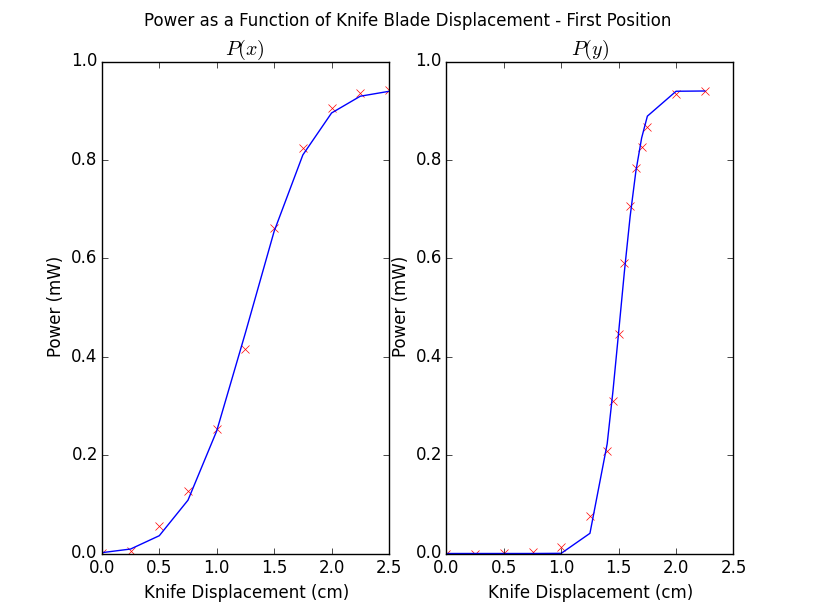
\includegraphics[scale = 0.5]{../Analysis/figure_1.png}\\
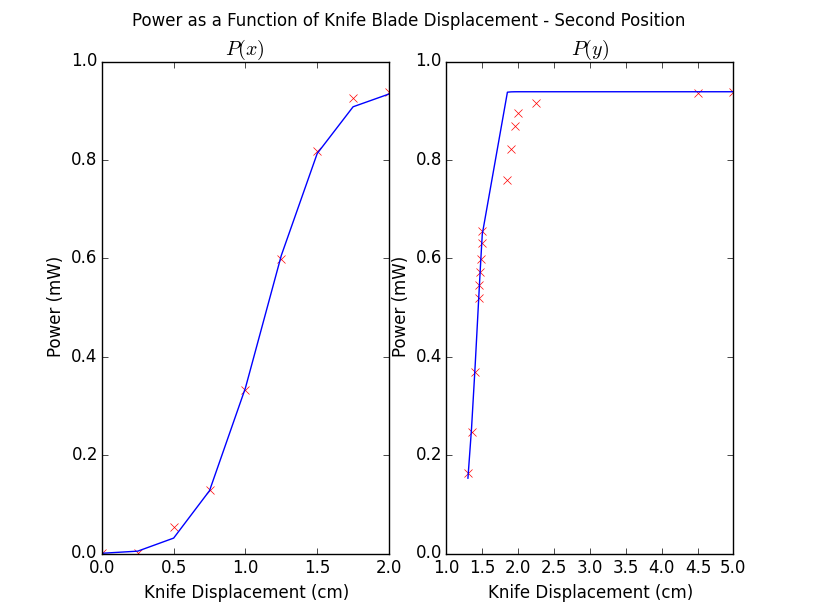
\includegraphics[scale = 0.5]{../Analysis/figure_2.png}
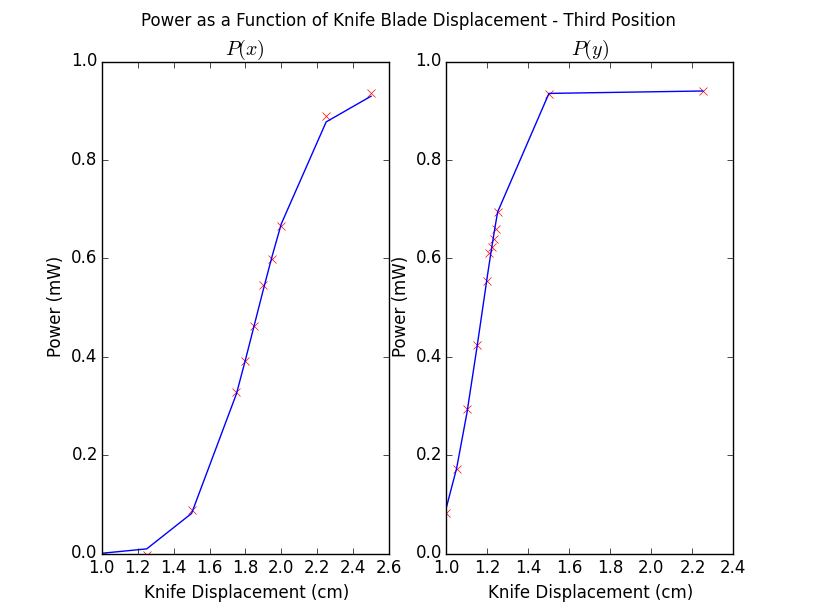
\includegraphics[scale = 0.5]{../Analysis/figure_3.png}
\caption{Figures Relevant to Part 4} 
\end{figure}
\noindent Rather than perform a full-blown F-test, however, simple comparison with the actual mean of the $x$-values allows us to roughly check how well our model is performing not due to the number of free parameters it has - large deviations of the mean (say, a threshold\footnote{This threshold is somewhat arbitrarily chosen, but tends to penalise the $y$-values unfairly. A fairer boundary is difficult to find.} of about 15\%) indicate problems with the data or the fit. 
\begin{table}
\centering
\begin{tabular}{|p{3cm}|p{3cm}|p{3cm}|p{3cm}|} 
\hline 
 & First Position ($z$ = 50 mm) & Second Position ($z$ = 436 mm) & Third Position ($z$ = 812 mm) \\ 
\hline 
$w_{x}$ & 0.877 & 0.679 & 0.517 \\ 
\hline 
$w_{y}$ & 0.299 & 0.270 & 0.258 \\ 
\hline 
Correction (x) & 1.276 & 1.123 & 1.851 \\ 
\hline 
Mean (x) & 1.250 & 1.000 & 1.795 \\ 
\hline 
Percent Diff. & 2.0\% & 12.3\% & 3\% \\ 
\hline 
Correction (y) & 1.508 & 1.432 & 1.166 \\ 
\hline 
Mean (y) & 1.287 & 2.021 & 1.283 \\ 
\hline 
Percent Diff. & 17\% & -28.5\% & 9.1\% \\ 
\hline
\end{tabular}
\caption{Minimum waist beams at different locations} 
\end{table}
\subsection*{Results}
\begin{figure}[H]
\centering
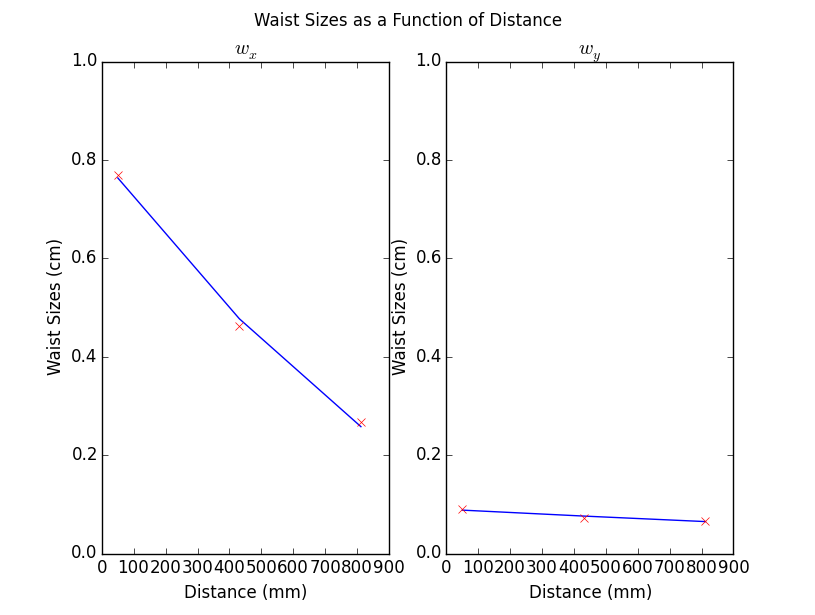
\includegraphics[width = \textwidth]{../Analysis/figure_4.png} 
\end{figure}
Our minimum waist sizes occur at:
\begin{itemize}
\item $w_{x} = 4.209\times 10^{-4}$ mm at $1869.49$ mm.
\item $w_{y} = 3.646\times 10^{-3}$ mm at $5406.45$ mm.
\end{itemize}
Are these reasonable? Most of the $y$-values exceed our 15\% threshold value, and our nonlinear  fit in $y$ for the second position is conspicuously far from several data points. I suspect that there was a lot of error involved in our $y$-value data collection - error functions should not resemble steep delta functions.\\
\\
No similar claim can be made for the $x$-values, which tend to be well-behaved.\\
\\
We took a card and explicitly measured the distance where the minimum waist appears to be found. Our results are that the minimum waist in $x$ is found at \textbf{1865} mm and the minimum waist in $y$ is at \textbf{872} mm. There is good agreement between our predicted and measured $w_{x}$, with less than 1\% difference; the same is not true for our measured and predicted $w_{y}$.
\begin{table}
\centering
\begin{tabular}{cccc}
\hline 
Predicted $w_{0x}$ Distance & Measured $w_{0x}$ Distance & Predicted $w_{0y}$ Distance & Measured $w_{0y}$ Distance \\ 
\hline 
1869 mm & 1865 mm & 5406 mm & 872 mm \\ 
\hline 
\end{tabular}
\caption{Predictions vs. Experiment for Part 5} 
\end{table}
\section*{Part 5: Numerically Calculating the Behavior of a Lens}
We chose a lens of focal length 53 mm, and numerically modeled it. Our T-matrix was obtained by multiplying
$$\begin{bmatrix}
  1 & d \\
  0 & 1 \\
\end{bmatrix}\begin{bmatrix}
  1 & 0 \\
  -\dfrac{1}{f} & 1 \\
\end{bmatrix} = \begin{bmatrix}
  1 - \dfrac{d}{f} & d \\
  -\dfrac{1}{f} & 1 \\
\end{bmatrix}$$
\begin{figure}[H]
\centering
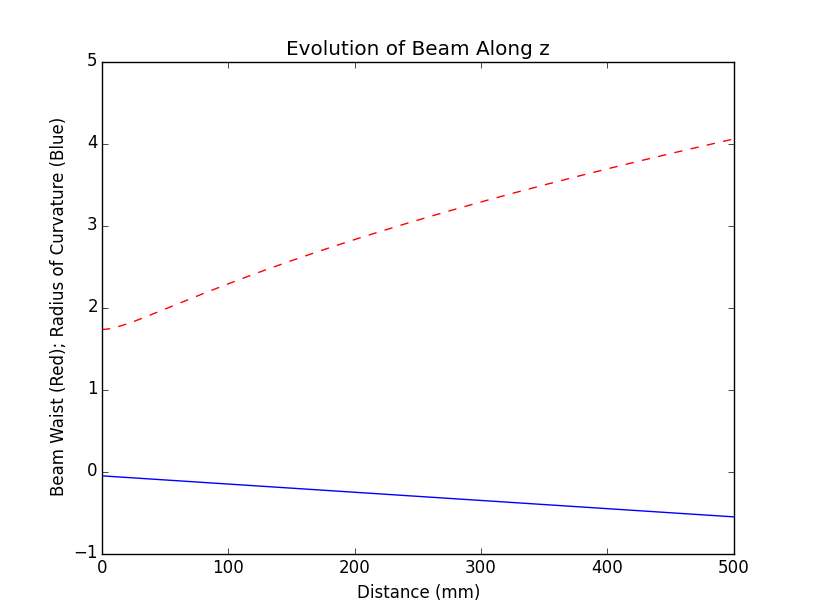
\includegraphics[width=\textwidth]{../Analysis/figure_5.png}
\caption{For $f$ = 53 mm} 
\end{figure}
\begin{figure}[H]
\centering
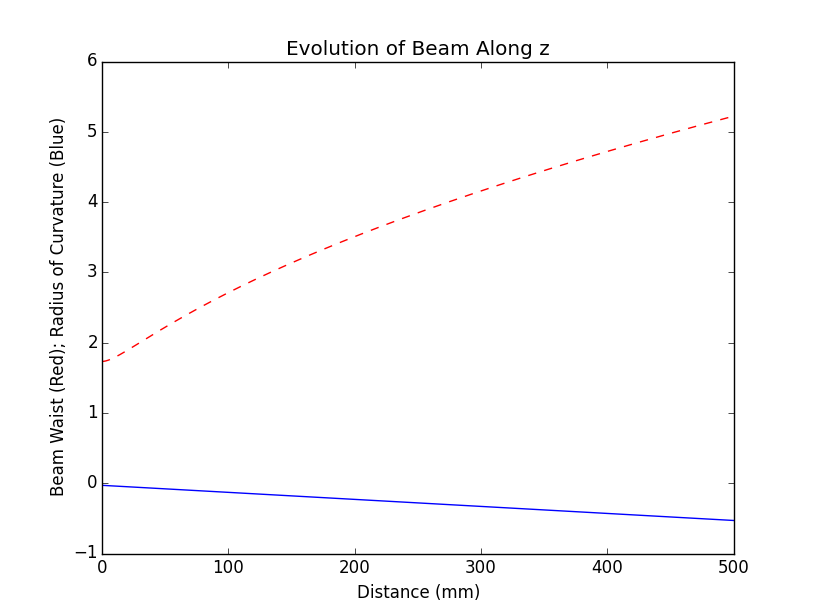
\includegraphics[width=\textwidth]{../Analysis/figure_6.png} 
\caption{For $f$ = 30 mm. Included for comparison with Figure 5.}
\end{figure}
\noindent We did not measure the actual minimum spot size, although we did measure where it occurred. The \textbf{minimum spot size} occurred at 80 mm from the head of the laser, or about 50 mm from the lens.\\
\\
Using the equation outlined in the lab manual i.e. $$z_{m} = \dfrac{f}{1 + \left(\dfrac{f\lambda}{\pi w_{01}^{2}}\right)^{2}} $$
, setting the wavelength equal to 635 nm, and discerning the relevant values of $w_{01}^{2}$ from Part 6, we obtain 
$$z_{my} = 52.999984167\;\mathrm{mm}$$
$$z_{mx} = 52.999999419\;\mathrm{mm}$$
which is approximately equal to the focal length anyway.

\section*{Part 6: Measuring the Effect of a Lens on a Beam}
We kept a lens of focal length 53 mm away from our lens, and worked out the beam profile at that point in a similar fashion to Part 4. 
\begin{figure}[h]
\centering
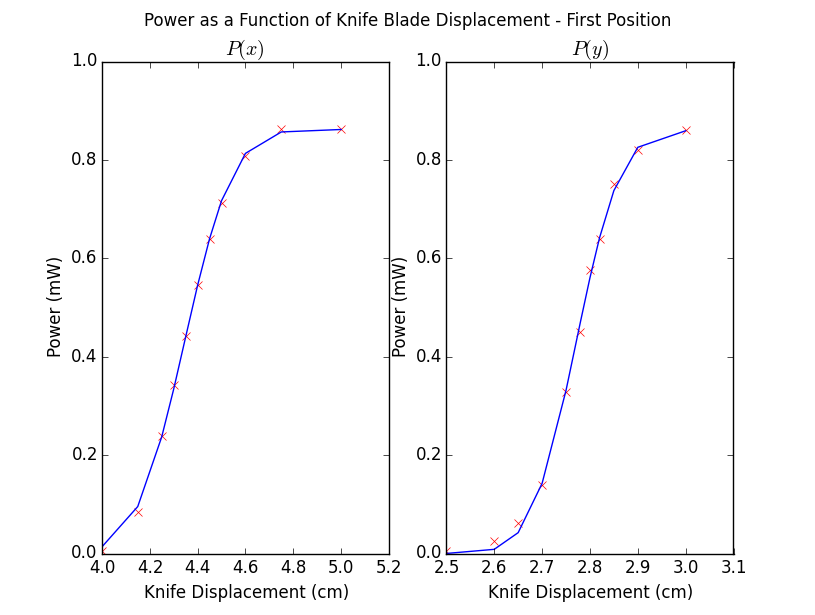
\includegraphics[scale =0.8]{../Analysis/figure_7.png}
\caption{Figure Relevant to Part 6. Red indicates the observed data; blue indicates our nonlinear fit to it.}
\end{figure}
\begin{table}[H]
\centering
\begin{tabular}{|c|c|c|c|c|c|c|c|}
\hline 
$w_{x}$ & Correction & Mean & Percent Diff. & $w_{y}$ & Correction & Mean & Percent Diff. \\ 
\hline 
0.32 & 4.34 & 4.43 & 2\% & 0.14 & 2.77 & 2.75 & 0.7\% \\ 
\hline 
\end{tabular}
\caption{Table relevant to Part 6}
\end{table}
\end{document}